En el \textit{algoritmo de Prim} también vamos a obtener un árbol de expansión de coste mínimo pero usando otra metodología.

Ahora, en vez de tener una partición donde se encuentran todos los vértices del grafo y se va cogiendo la arista con menor valor, vamos a tener un vector de booleanos \(U\) que indicará porqué vértices hemos pasado y se empezará desde el vértice con menor coste.

\begin{figure}[h]
  \begin{center}
    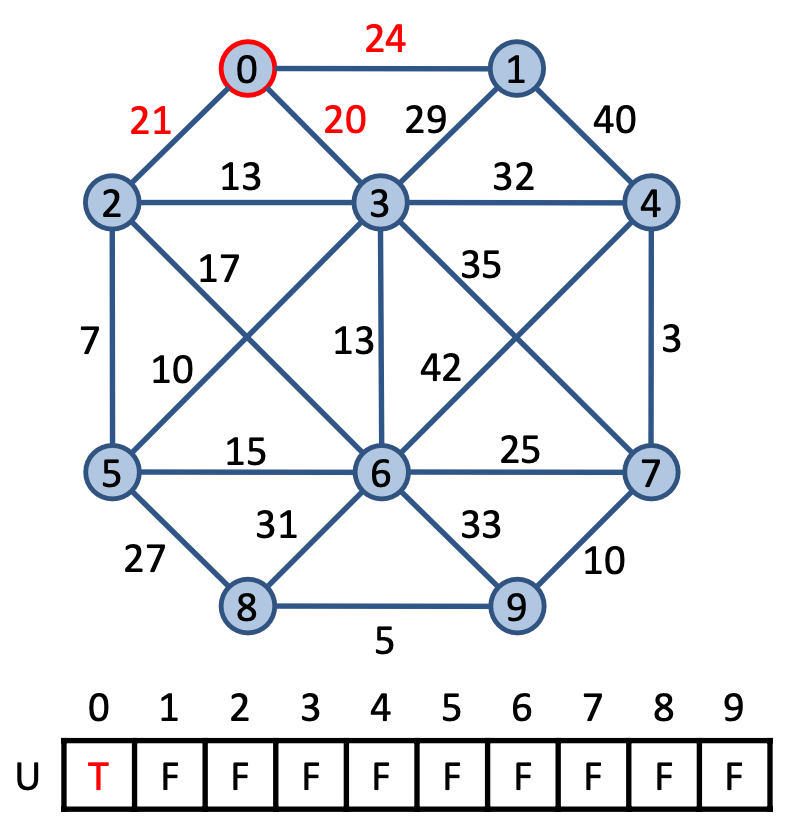
\includegraphics[width=.5\textwidth]{assets/prim1.png}
  \end{center}
  \caption{Ejemplo del algoritmo Prim}
\end{figure}
\newpage
Vemos que partimos desde el vértice con valor 0 y que tenemos 3 aristas disponibles con costes (20, 21 y 24), lo que vamos a hacer es pasar por la arista que tenga menor coste, es decir, por la de coste 20 uniendo los vértices (0 y 3) y las otras dos restantes quedaría `eliminadas'.

\begin{figure}[h]
  \begin{minipage}{0.4\textwidth}
    \centering
    \begin{subfigure}{\textwidth}
      \centering
      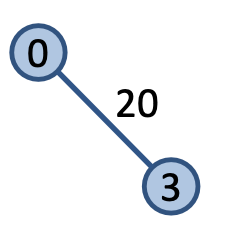
\includegraphics[width=.5\textwidth]{assets/prim2.png}
      \caption{Unimos ambos vértices con la arista de menor coste.}
    \end{subfigure}
  \end{minipage}
  \hfill
  \begin{minipage}{0.5\textwidth}
    \centering
    \begin{subfigure}{\textwidth}
      \centering
      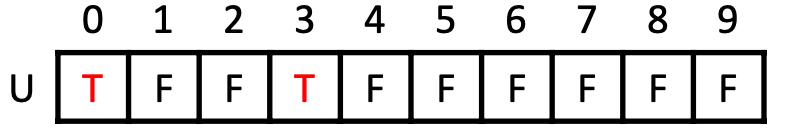
\includegraphics[width=\textwidth]{assets/prim3.png}
      \caption{Ponemos en T (true) los vértices por los que hemos pasado.}
    \end{subfigure}
  \end{minipage}
  \caption{Ejemplo 1 Prim}
\end{figure}

Ahora nos encontramos en el vértice `3' y si nos fijamos en el grafo de la \textit{Figura 10.17} vemos que se puede unir con varios vértices (\(3 \leftrightarrow 2\) con coste 13), (\(3 \leftrightarrow 6\) con coste 13) y (\(3 \leftrightarrow 5\) con coste 10), como la arista de menor coste es 10, uniremos (\(3 \leftrightarrow 5\)).

\begin{figure}[h]
  \begin{minipage}{0.4\textwidth}
    \centering
    \begin{subfigure}{\textwidth}
      \centering
      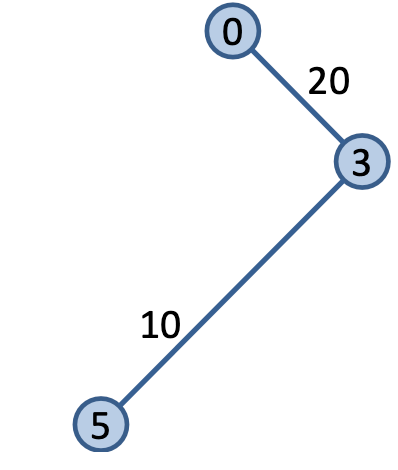
\includegraphics[width=.5\textwidth]{assets/prim5.png}
      \caption{Unimos 3 y 5.}
    \end{subfigure}
  \end{minipage}
  \hfill
  \begin{minipage}{0.5\textwidth}
    \centering
    \begin{subfigure}{\textwidth}
      \centering
      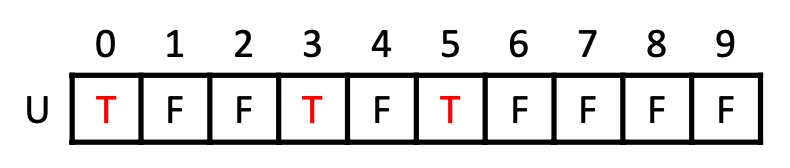
\includegraphics[width=.8\textwidth]{assets/prim6.png}
      \caption{Ponemos en T (true) en el vértice 5.}
    \end{subfigure}
  \end{minipage}
  \caption{Ejemplo 2 Prim}
\end{figure}

Ahora encontramos un problema, tras haber unido los vértices (2 y 5) nos encontramos en el vértices `2', pero no podemos unirlo con nigún vertice ya que si lo unimos con los vértices (0,3) tendríamos un ciclo.
\begin{figure}[h]
  \begin{minipage}{0.4\textwidth}
    \centering
    \begin{subfigure}{\textwidth}
      \centering
      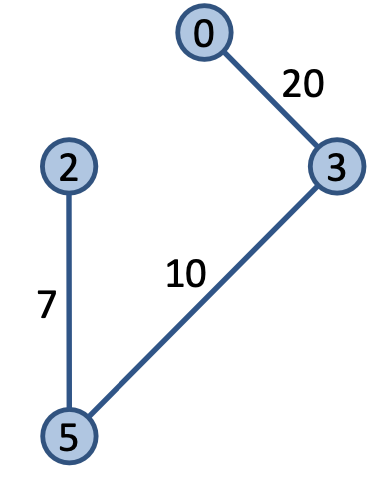
\includegraphics[width=.5\textwidth]{assets/prim9.png}
    \end{subfigure}
  \end{minipage}
  \hfill
  \begin{minipage}{0.5\textwidth}
    \centering
    \begin{subfigure}{\textwidth}
      \centering
      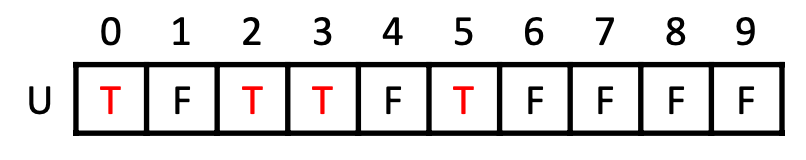
\includegraphics[width=.8\textwidth]{assets/prim10.png}
    \end{subfigure}
  \end{minipage}
  \caption{Ejemplo 3 Prim}
\end{figure}
\newpage
Si nos fijamos en el grafo de ejemplo (\textit{Figura 10.17}) vamos que el vértice 2 se puede unir con el 6 (\(2 \leftrightarrow 6\) con coste 17), pero es que el vértice 3 también se puede unir con 6 (\(3 \leftrightarrow 6\) con coste 13), como el coste de este último es menor, saltamos del vértice 2 al 3 y unimos con el vértice 6.

\begin{figure}[h]
  \begin{minipage}{0.4\textwidth}
    \centering
    \begin{subfigure}{\textwidth}
      \centering
      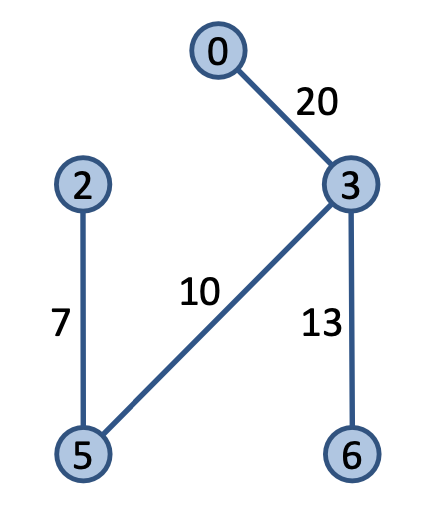
\includegraphics[width=.5\textwidth]{assets/prim11.png}
      \caption{Unimos 3 y 6}
    \end{subfigure}
  \end{minipage}
  \hfill
  \begin{minipage}{0.5\textwidth}
    \centering
    \begin{subfigure}{\textwidth}
      \centering
      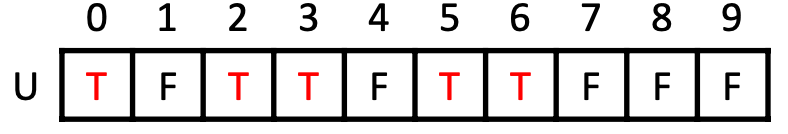
\includegraphics[width=.8\textwidth]{assets/prim12.png}
      \caption{Ponemos en T (true) en el vértice 6.}
    \end{subfigure}
  \end{minipage}
  \caption{Ejemplo 4 Prim}
\end{figure}

Ahora vemos que podemos unir los vertices 6 y 7 (\(6 \leftrightarrow 7\) con coste 25), pero también podemos saltar al vértice 0 y unirlo con 1 (\(0 \leftrightarrow 1\) con coste 24), como la arista de éste último tiene menor coste y por tanto, se unen primero dichos vértices y luego unimos 6 con 7.
\begin{figure}[h]
  \begin{minipage}{0.4\textwidth}
    \centering
    \begin{subfigure}{\textwidth}
      \centering
      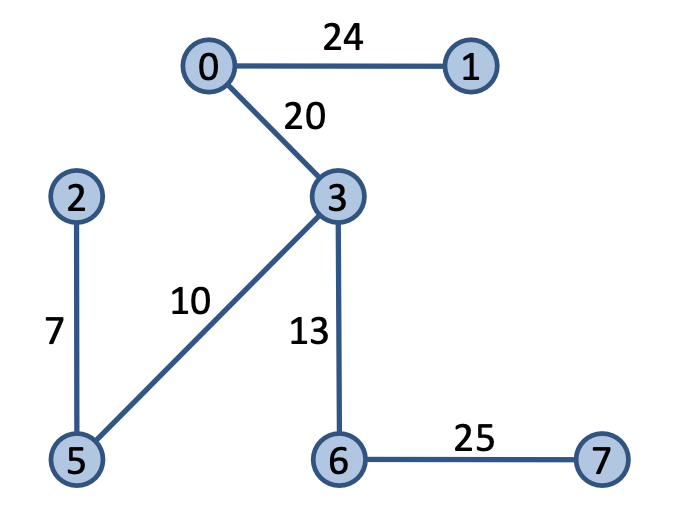
\includegraphics[width=.5\textwidth]{assets/prim13.png}
      \caption{Unimos primero 0 y 1 y luego 6 y 7.}
    \end{subfigure}
  \end{minipage}
  \hfill
  \begin{minipage}{0.5\textwidth}
    \centering
    \begin{subfigure}{\textwidth}
      \centering
      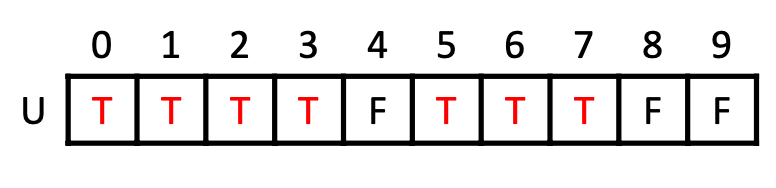
\includegraphics[width=.8\textwidth]{assets/prim14.png}
      \caption{Ponemos en T (true) en el vértice 1 y 7.}
    \end{subfigure}
  \end{minipage}
  \caption{Ejemplo 5 Prim}
\end{figure}

Seguimos uniendo vértices teniendo en cuenta el peso de las aristas y tenemos como resultado final:
\begin{figure}[h]
  \begin{minipage}{0.4\textwidth}
    \centering
    \begin{subfigure}{\textwidth}
      \centering
      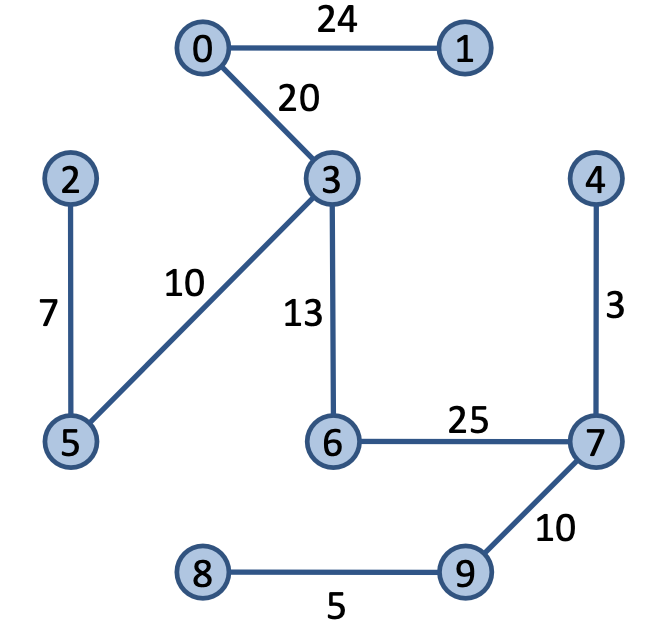
\includegraphics[width=.5\textwidth]{assets/prim15.png}
      \caption{Todos los nodos unidos sin ciclos.}
    \end{subfigure}
  \end{minipage}
  \hfill
  \begin{minipage}{0.5\textwidth}
    \centering
    \begin{subfigure}{\textwidth}
      \centering
      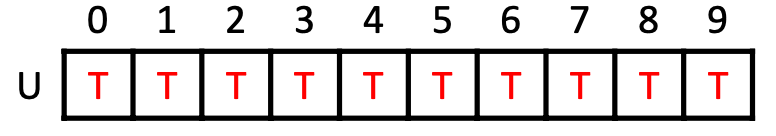
\includegraphics[width=.8\textwidth]{assets/prim16.png}
      \caption{Vector de booleano con todos a T (true).}
    \end{subfigure}
  \end{minipage}
  \caption{Resultado ejemplo de algoritmo Prim}
\end{figure}

Como vemos en las figuras (\textit{Figura 10.17: Resultado ejemplo algoritmo Kruskal}) y (\textit{Figura 11.24: Resultado ejemplo algoritmo Prim}) ambos grafos son idénticos, sin embargo, pueden existir casos en que sean diferentes.

Esto es debido a que aunque Kruskal y Prim trabajen con metodologías diferentes pueden devolver el mismo \textit{árbol de expansión de coste mínimo}, ya que al estar uniendo vértices cuya aristas son las de menor coste es muy probable que el resultado sea el mismo.

Es decir, \textit{Kruskal} y \textit{Prim} hacen lo mismo pero de menera diferente.